\documentclass[aspectratio=169]{beamer}
\usepackage[T1]{fontenc}
\usepackage{graphicx}
\usepackage{tikz}
\usetikzlibrary{positioning}

\usetheme{default}
\setbeamertemplate{navigation symbols}{}
\setbeamertemplate{footline}{}
\setbeamercolor{background canvas}{bg=white}

\begin{document}

% 1 -- completely black
{
  \setbeamercolor{background canvas}{bg=black}
  \begin{frame}[plain]
  \end{frame}
}

% 2 -- soccer field sketch with audience
\begin{frame}[plain]
  \centering
  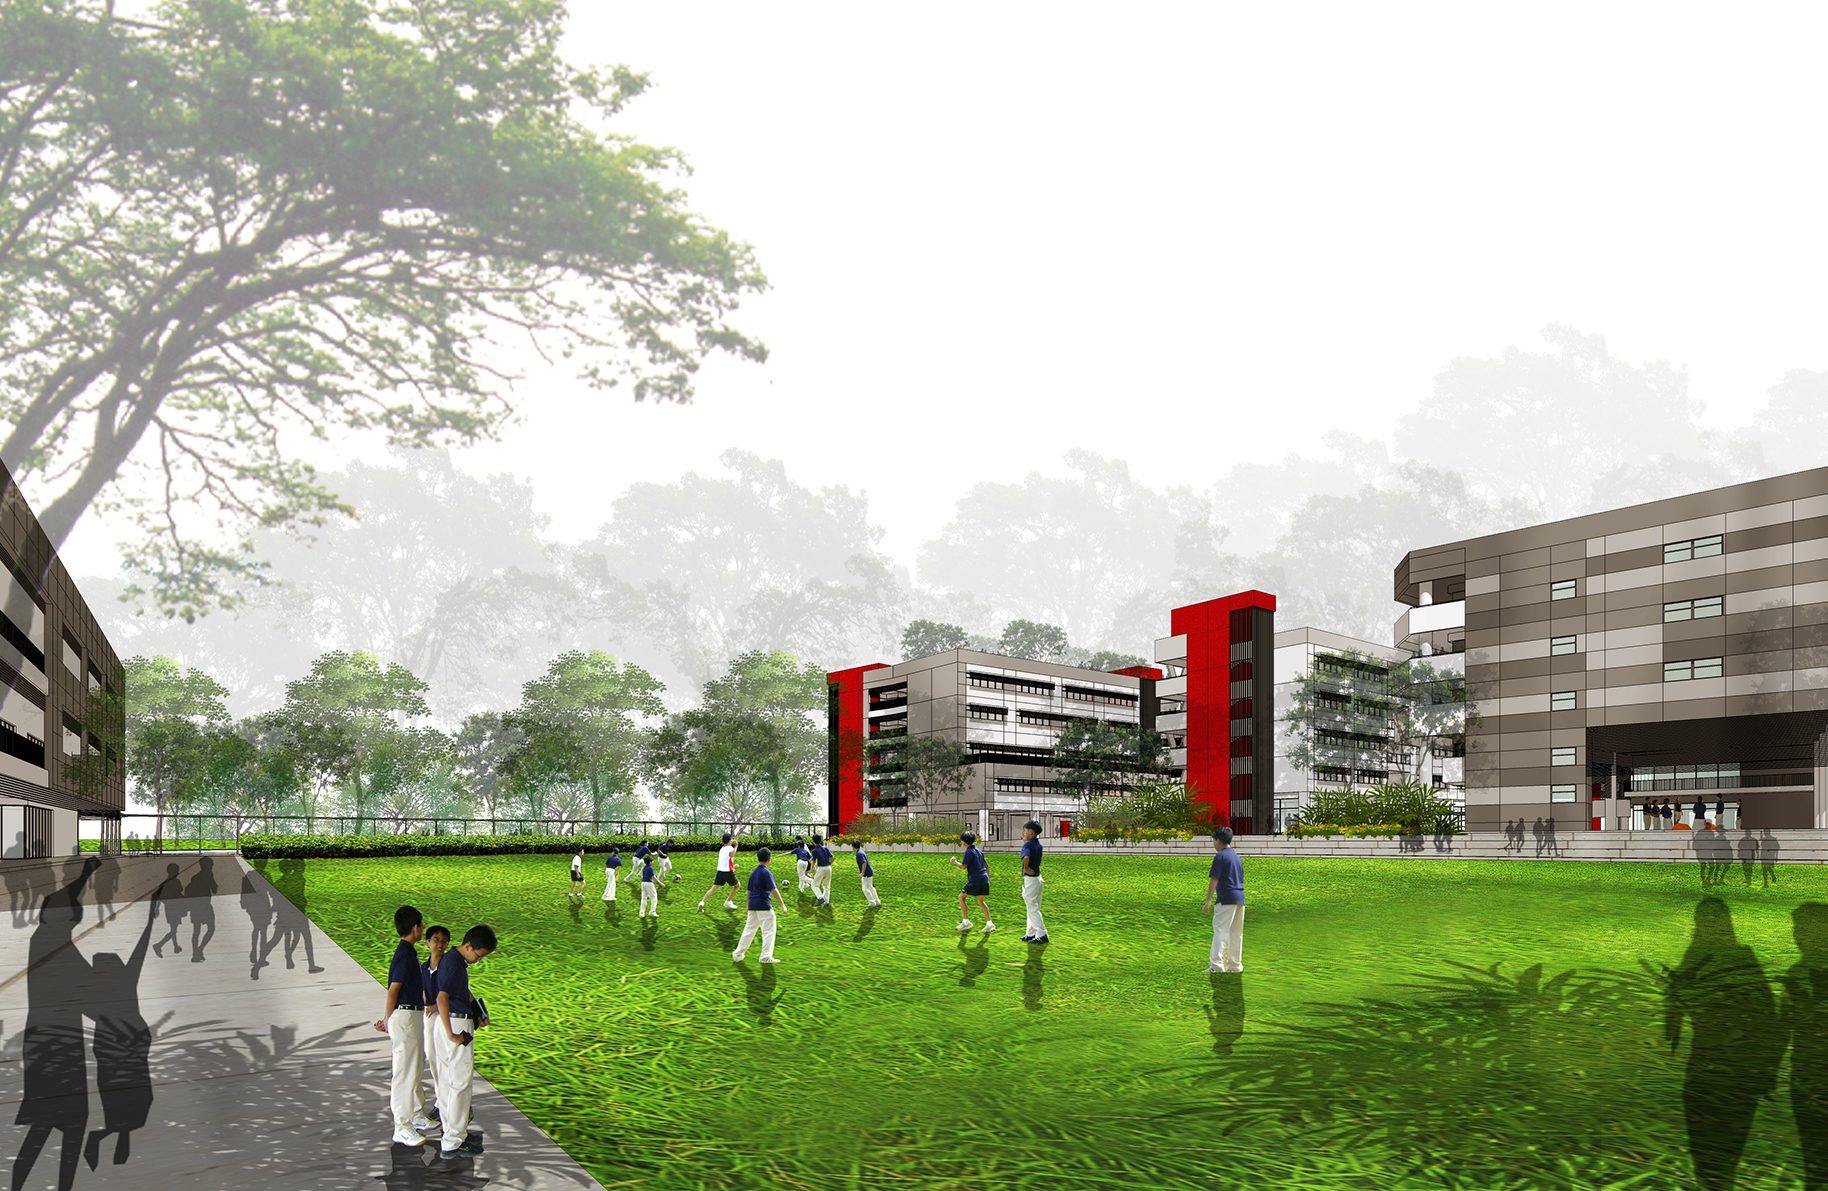
\includegraphics[width=\paperwidth,height=\paperheight,keepaspectratio]{images/soccer.jpg}
\end{frame}

% 3 -- observables of ATLAS
\begin{frame}{What observables does ATLAS have?}
  \centering
  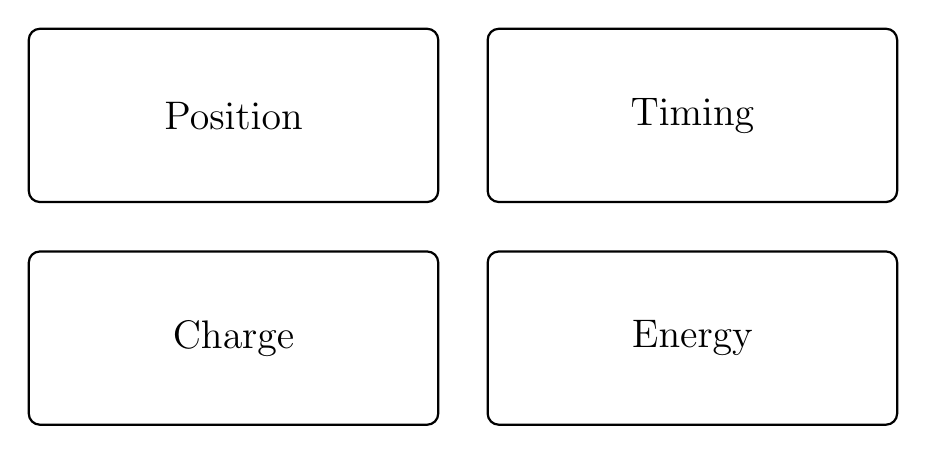
\begin{tikzpicture}[
      box/.style={draw, rounded corners, minimum width=5.2cm, minimum height=2.2cm,
                  align=center, font=\Large, thick}]
    \node[box] (a) {Position};
    \node[box, right=0.6cm of a] (b) {Timing};
    \node[box, below=0.6cm of a] (c) {Charge};
    \node[box, right=0.6cm of c] (d) {Energy};
  \end{tikzpicture}
\end{frame}

% 4 -- technical drawing of (part of) the ATLAS detector
\begin{frame}[plain]
  \centering
  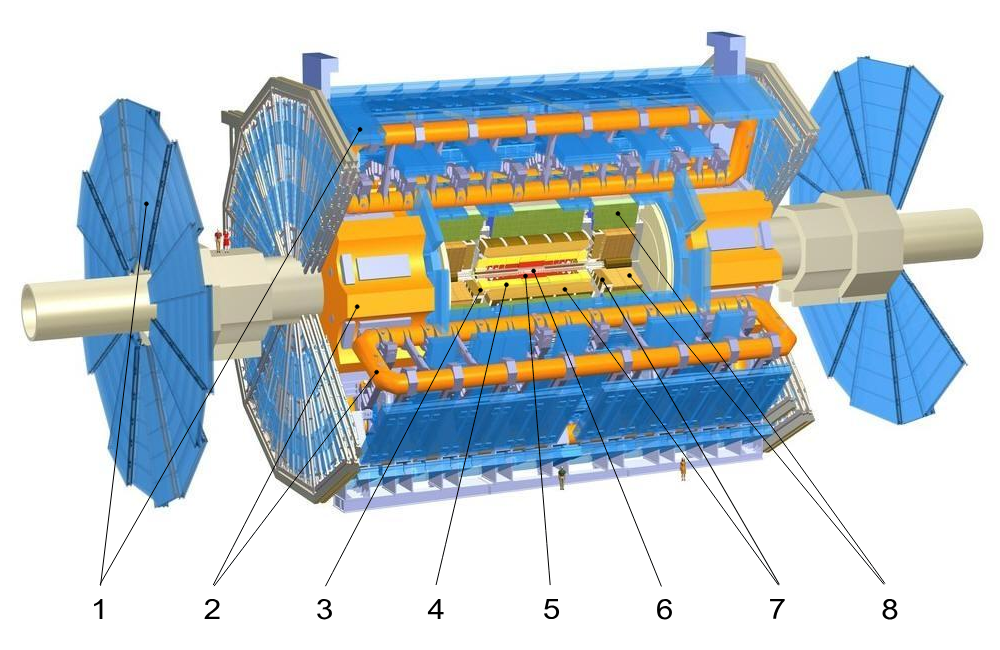
\includegraphics[width=\paperwidth,height=\paperheight,keepaspectratio]{images/detector.png}
  \begin{tikzpicture}[remember picture, overlay]
    \node[anchor=north east, fill=white, fill opacity=0.8, text opacity=1, inner sep=3pt]
      at (current page.north east) {\footnotesize\href{https://atlas-viewer.web.cern.ch}{atlas-viewer.web.cern.ch}};
  \end{tikzpicture}
\end{frame}

% 5 -- reconstructed tracks
\begin{frame}[plain]
  \centering
  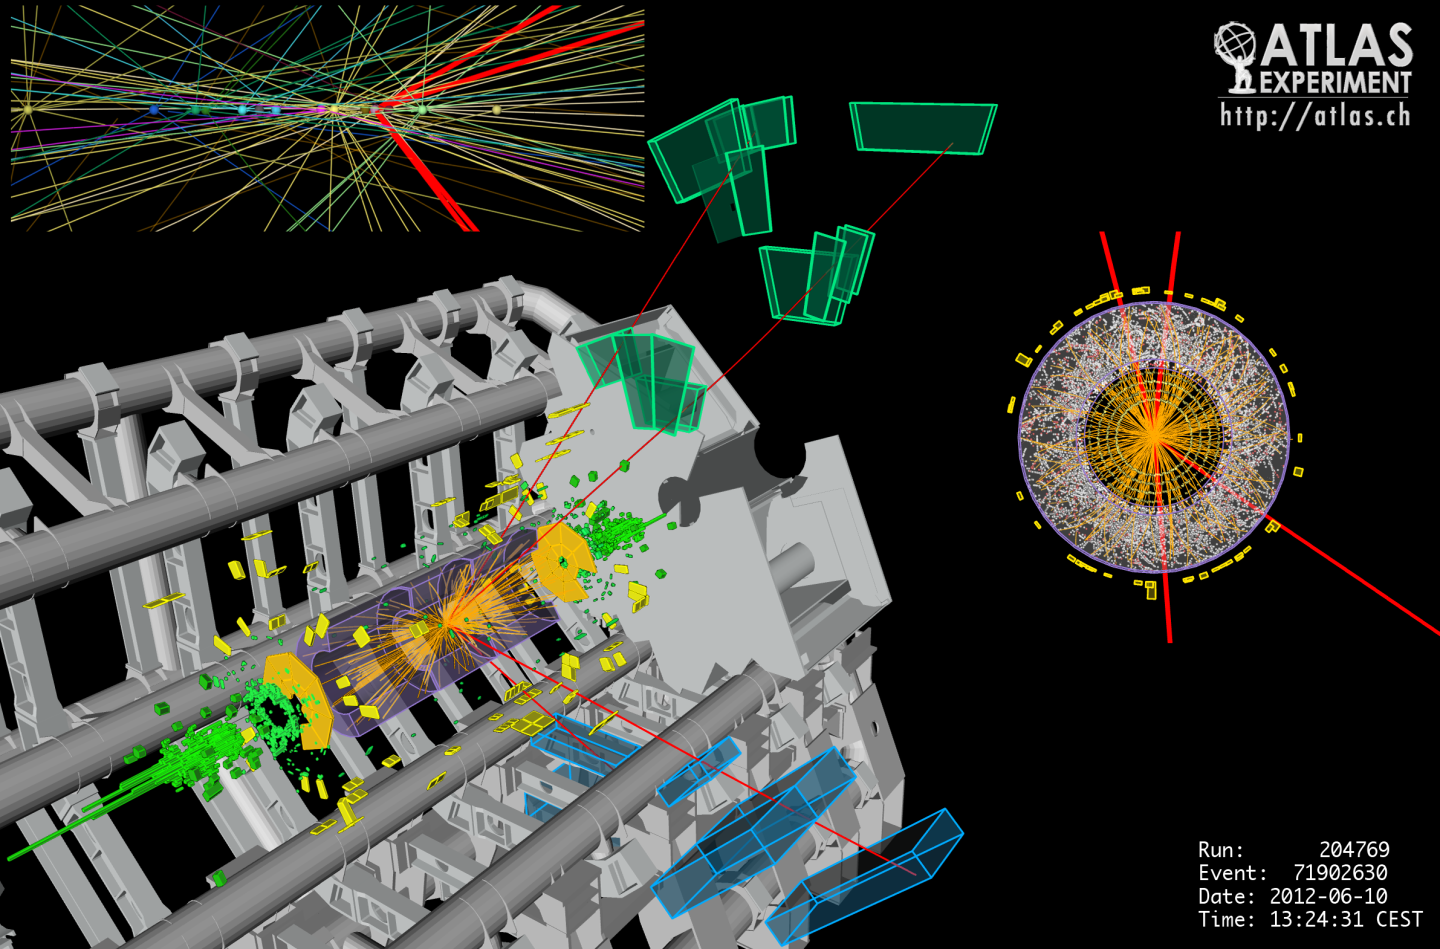
\includegraphics[width=\paperwidth,height=\paperheight,keepaspectratio]{images/tracks.png}
\end{frame}

\end{document}
